\section{RESULTADOS}

\subsection{Invasibilidad}

Para una zona $Z$ en particular definimos la \emph{zona relativa} al tipo de comunidad $n$ como $Z_n = Z \cap C_n$. \\
A continuaci\'on se describen resultados para la combinaci\'on de estrategias de forrajeo \emph{Grazing-Grazing-Active}. Dado que en los otros dos casos se obtiene una respuesta cualitativa similar estos no ser\'an detallados.

\subsubsection{$ C \to R$}
Se observa un aumento en el \'area total de $Z(I_{\C \to \R})$ con respecto a aumentos en $m_P$ y $k_0$ teniendo ambos una respuesta cualitativa similar(i.e cualitativamente el cambio respecto a aumentos en $k_0$ para un valor fijo de $m_P$ es similar al cambio respecto a aumentos en $m_P$ para un valor fijo de $k_0$)\\
Adem\'as dicho aumento se debe principalmente a aumentos en el \'area de las zonas relativas $1 , 2 y 6$ es decir conforme aumenta la masa del depredador tope, la proporci\'on de comunidades con $k_{\RP} <1 : C_1,C_2$ y $C_6$ donde se da este tipo de invasi\'on aumenta.\\ 
El par\'ametro $\phi$ controla principalmente el borde superior de la zona, restringuiendo valores elevados de $k_{\RC}$ a valores altos de $\phi$, para el valor de $2$ obtenemos una forma de $V$ centrada alrededor de $k_0 = 0$ donde el l\'imite superior aumenta con $k_{\CP}$.\\
La dimensi\'on del \'area de busqueda afecta el \'area total de las zonas, siendo mayor en el caso $3D$. 

\begin{figure}
  \centering
  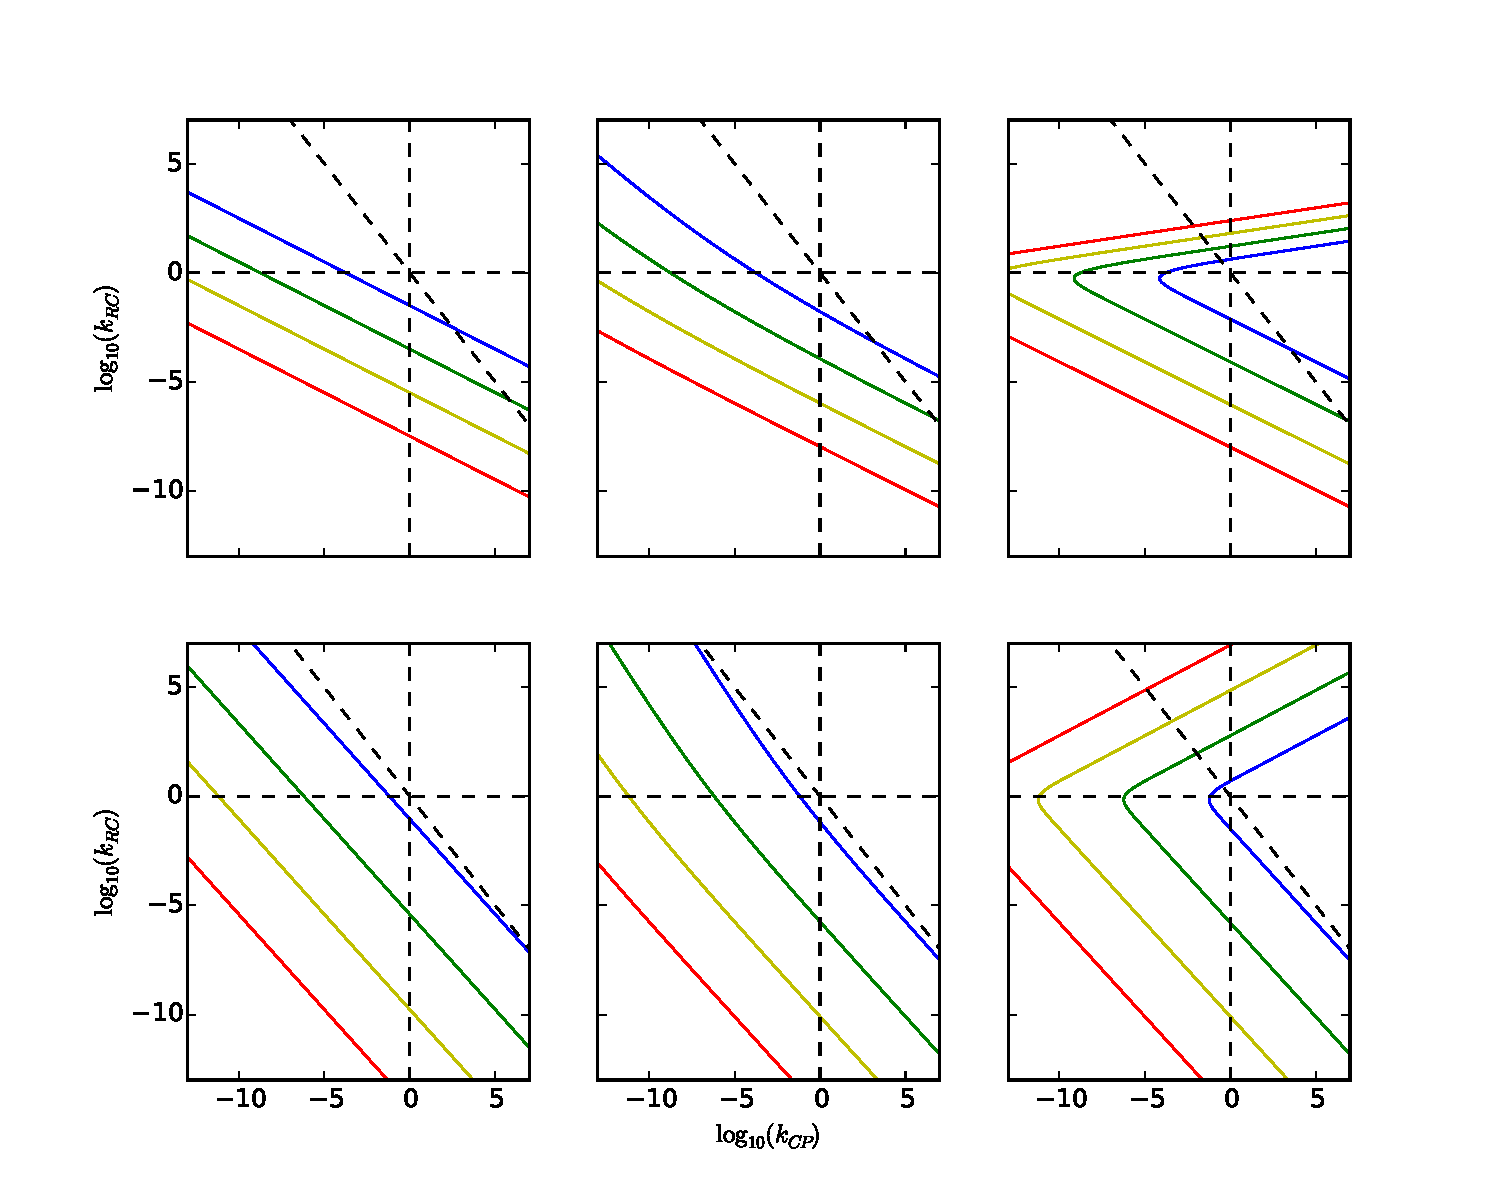
\includegraphics[width = 0.99\textwidth]{./Plots/Z(IC2)AcGrGr.pdf}
  \caption[Env $Z(IC2)$]{\emph{Envolturas de Invasibilidad} para el caso de el depredador intermedio $C$ como invasor frente a una comunidad receptora formada por $R$. La fila superior es para espacios de b\'usqueda bidimensionales y la inferior tridimensionales, las columnas de izquierda a derecha aumentan el valor de $\phi$, siendo $0.02,0.2$ y $2$ respectivamente.Las diferentes lineas implican distintas masas de depredador $m_P$ :({\hwplotR}) $10^5 kg$,  ({\hwplotY}) $1kg$, ({\hwplotG}) $10^{-5}kg$ y ({\hwplotB}) para $10^{-10}kg$. ({\hwplotK}) separa las zonas donde $K_{RC},K_{CP},k_{RP}$ son mayores o menores que 1 respectivamente. $k_0 = 0.1$ y $k_0 = 30$ para el caso $2D$ y $3D$ respectivamente, los valores de los otros par\'ametros son los descritos en el anexo \ref{subsec:params}}
  \label{fig:Z(IC2)}
\end{figure}

\subsubsection{$ P  \to R$}

De forma similar al caso anterior se observa un aumento en el \'area total de $Z(I_{\PP \to \R})$ conforme aumenta tanto $k_0$ como $m_p$ y el cambio es similar en ambos casos. Se observa que los bordes de la zona estan determinados por $k_{\RP}$ y conforme aumenta $m_p$($k_0$) es menor el valor necesario para que se de la invasi\'on, es decir el crecimiento respecto a $m_P$($k_0$) no es uniforme sino esta direccionado a comunidades con $k_{\RP} < 1 $ \\
El valor de $\phi$ limita la inclusi\'on de valores elevados de $k_{\RP}$ dentro de la zona , y para $\phi = 2$ tenemos que la zona esta compuesta por una franja incluida entre 2 valores de $k_{\RP}$.\\
Igual que en el caso anterior la dimensi\'on del espacio de b\'usqueda afecta el \'area total de la zona, y es mayor para ambientes $3D$.

\begin{figure}
  \centering
  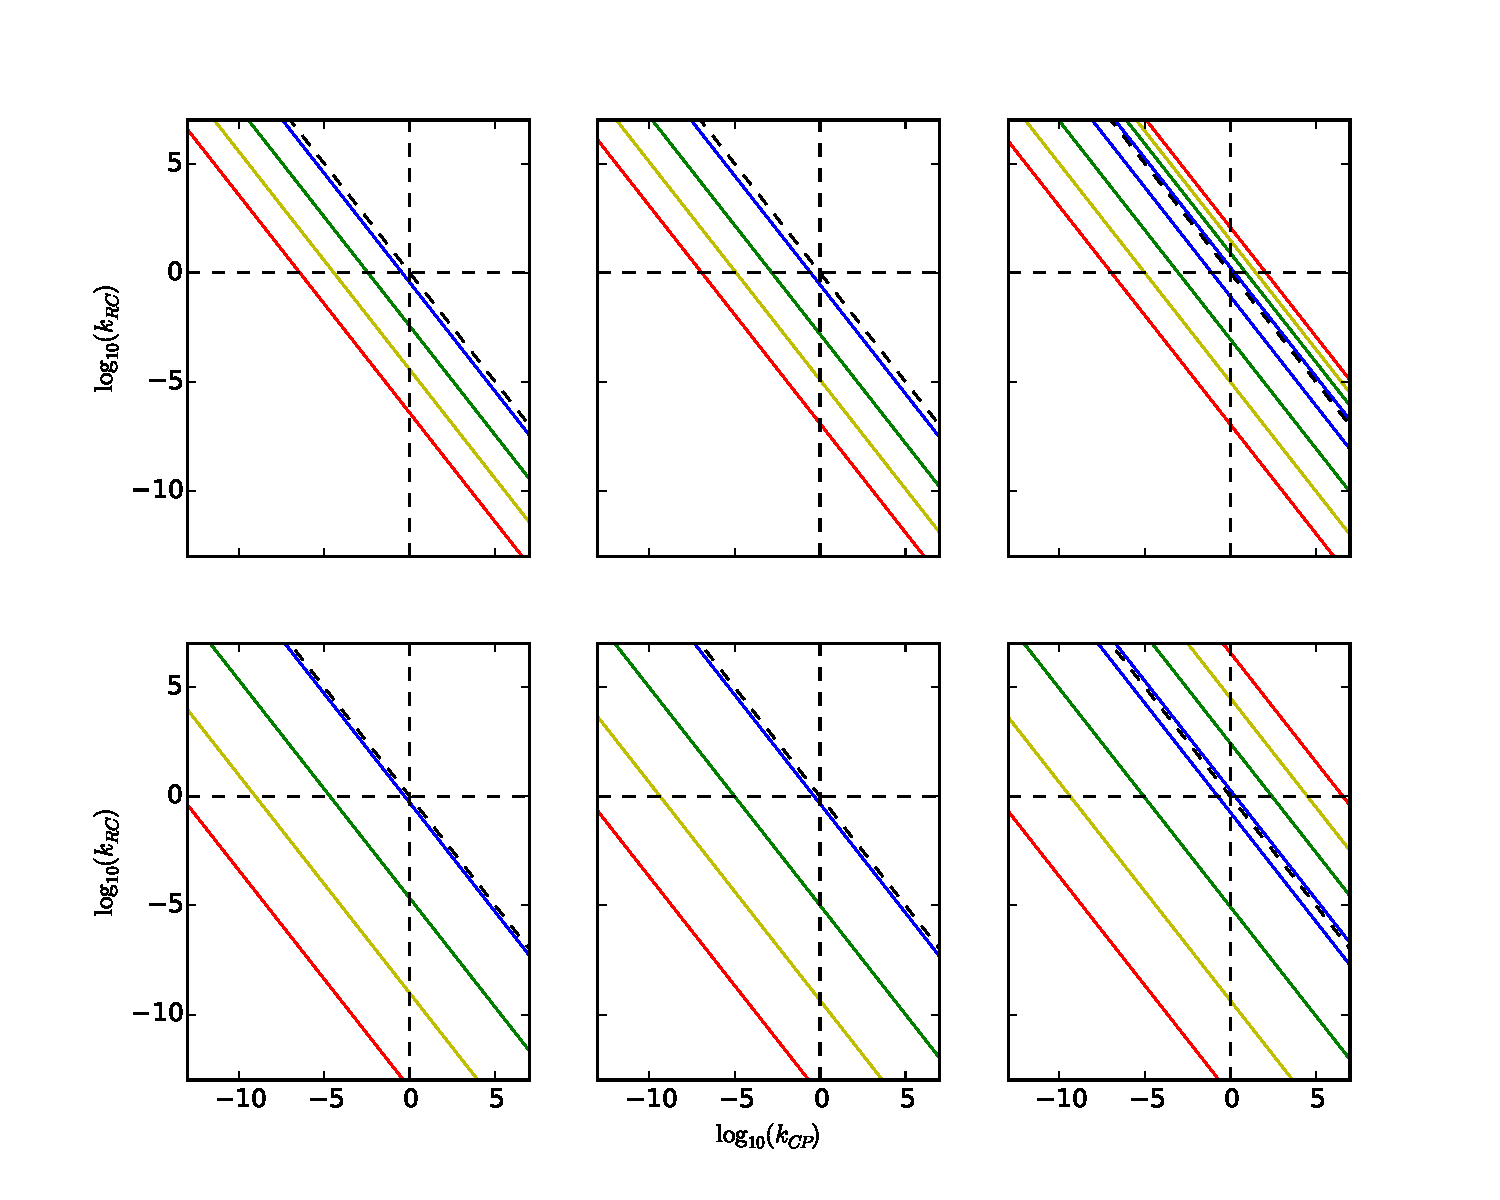
\includegraphics[width = 0.99\textwidth]{./Plots/Z(IC3)AcGrGr.pdf}
  \caption[Env $Z(IC2)$]{\emph{Envolturas de Invasibilidad} para el caso de el depredador intermedio $P$ como invasor frente a una comunidad receptora formada por $R$.Las dem\'as especificaciones se comparten con la figura ~\ref{fig:Z(IC2)}}
  \label{fig:Z(IC3)}
\end{figure}


\subsubsection{$ P \to R-C$}

En todos los casos explorados $Z(I_{\PP \to \R - \C})$ tiende a crecer con respecto a aumentos en la masa del depredador $m_P$, y adem\'as forman una secuencia encajante, igual que en los casos anteriores se observa una respuesta cualitativa similar en cambios respecto a $m_p$ y $k_0$. Sin embargo el crecimiento no es uniforme, las zonas relativas si bien tienden a crecer lo hacen de manera desigual dependiendo adem\'as del valor del par\'ametro $\phi$.\\

El valor de $\phi$ controla en cierta la ``forma'' de $Z(I_{\PP \to \R - \C})$, observandose por lo general una relaci\'on inversa del valor de $phi$ y el \'area total de $Z(I_{\PP \to \R - \C})$ irrespectivamente de la masa. Sin embargo afecta de manera desigual los distintos tipos de Comunidades.\\ Por ejemplo, en el caso de comunidades con distribuci\'on de masa $C_1$ el par\'ametro es pr\'acticamente irrelavante sobre la zona relativa $Z(I_{\PP \to \R - \C})_1$, y por el contrario para comunidades $C_5$ el cambio es dram\'atico, dado que entre $\phi  = 0.02 - 2$, $Z(I_{\PP \to \R - \C})_5$ pasa de ser no vac\'ia y cubrir en su totalidad(en el caso $3D$) a $C_5$ (i.e $Z(I_{\PP \to \R - \C})_5 = C_5$) para todas las masas $m_P$ exploradas, a ser vac\'io para todo $m_P$ en el segundo caso.\\
La dimensi\'on del espacio de b\'usqueda afecta el \'area total y las \'areas relativas de $Z(I_{\PP \to \R - \C})$.\\
En el primer caso observamos que generalmente es mayor en espacios tridimensionales(3D) y esta diferencia se acent\'ua conforme la masa $m_P$ aumenta,en el segundo  tenemos un patr\'on muy similar pero en este caso para $m_P$ bajos se pueden observar comunidades donde el \'area de la zona relativa es mayor en ambientes bidimensionales, como por ejemplo $Z(IC_3)$ para $m_P = 10^{-10}$. \\
Algo que resaltar es que el borde inferior(en escala logar\'itmica) tiende a ser \emph{paralelo} a $(\log_{10}(K_{CP}),-log_{10}(K_{RC}))$ para espacios de b\'usqueda $3D$ y no en el caso $2D$


\begin{figure}
  \centering
  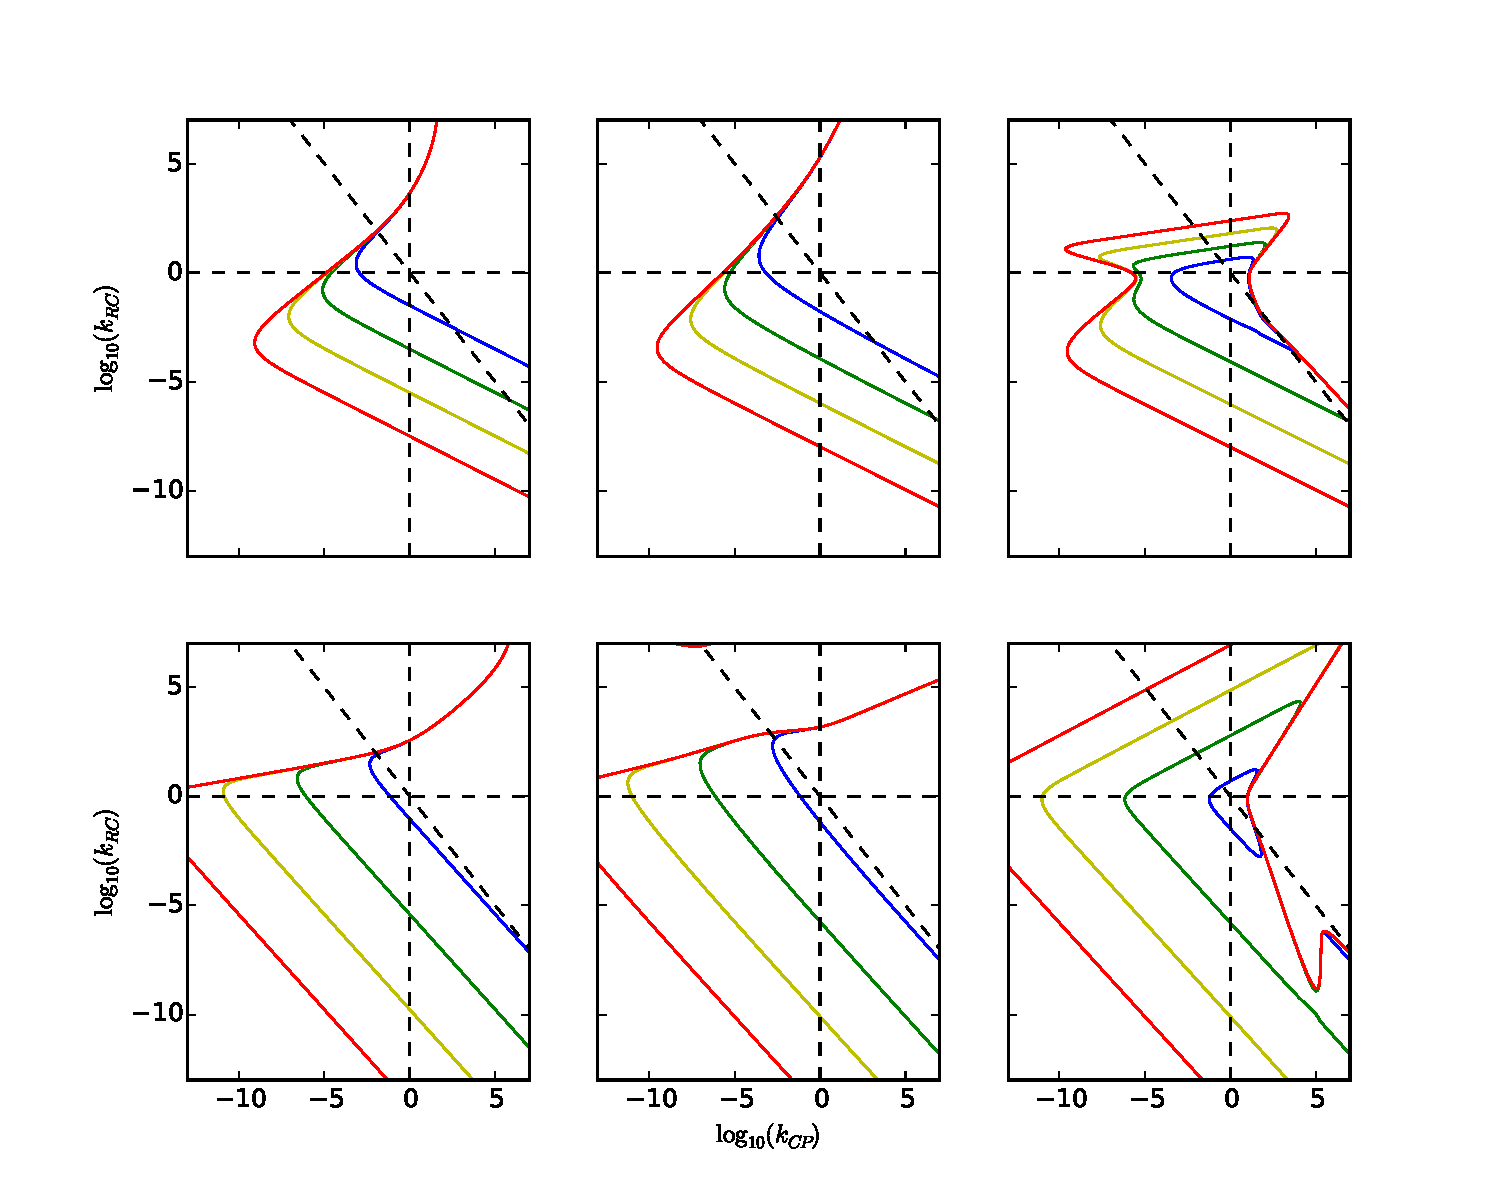
\includegraphics[width = 0.99\textwidth]{./Plots/Z(IC4)AcGrGr.pdf}
  \caption[Env $Z(IC4)$]{\emph{Envolturas de Invasibilidad} para el caso de el depredador tope $P$ como invasor frente a una comunidad receptora formada por $R-C$ .Las dem\'as especificaciones se comparten con la figura ~\ref{fig:Z(IC2)}}
  \label{fig:Z(IC4)}
\end{figure}

\subsubsection{$C \to R-P$}
De forma similar al caso anterior tenemos que el \'area total de $Z(I_{\C \to \R - \PP})$ esta relacionada positivamente con el valor de $m_P$ y $k_0$, sin embargo a diferencia del caso anterior las zonas para distintos $m_P$ si bien tienen intersecci\'on no vac\'ia ,no estan incluidas una en otra. Es decir a parte de crecimiento tenemos un desplazamiento conforme aumenta $m_P$. \\

En este caso es bastante notoria la no uniformidad en el \'area de las zonas relativas.\\

El par\'ametro $\phi$ juega un papel importante en la topolog\'ia de $Z(I_{\C \to \R - \PP})$, para valores peque\~nos el conjunto es conexo, sin embargo para $\phi = 2$(y $m_p>10^{-10}$ y $k_0 > 3$ en el caso $3D$) el conjunto tiene 2 componentes $\vartheta_C^1$ y $\vartheta_C^2$ . La distancia entre estas componenes aumenta con $m_P$ y $k_0$ ; podemos distinguirlas por el hecho que una de ellas $\vartheta_C^1$ intersecta principalmente las zonas $C_3,C_4,C_5$ y la otra $\vartheta_C^2$ las zonas $C_1,C_2,C_6$, es decir se caracterizan por contener comunidades con $k_{\RP} >1 $($\vartheta_C^1$) o $k_{\RP}<1$ ($\vartheta_C^2$). Siendo la primera la que presenta mayor \'area. \\
Para $\phi = 0.2 ,0.02$  tenemos que $Z(I_{\C \to \R - \PP})$ intersecta principalmente a las zonas $C_2,C_3$(Comunidades con $k_{\RC}>1$ y$k_{\CP} <1$) y posee una ``\emph{cola}'' que es paralela(en escala logar\'itmica) a $\log_{10}(K_{CP}) = -log_{10}(K_{RC})$ y que dependiendo del valor de $m_P$($k_0$) esta contenido en las zonas $C_1,C_2,C_6$ o $C_3,C_4,C_5$, es decir $k_{RP} > 1$ o $k_{RP}<1$. \\

La dimensi\'on del espacio de b\'usqueda igual que en el caso anterior afecta el \'area total de $Z(I_{\C \to \R - \PP})$ la cual es mayor en ambientes tridimensionales.\\
Para $\phi = 2$ se observa que el \'area de $\vartheta_C^2$ es por lo general mayor en ambientes bidimensionales y lo contrario ocurre con el otro componente en ambientes 3D.

\begin{figure}
  \centering
  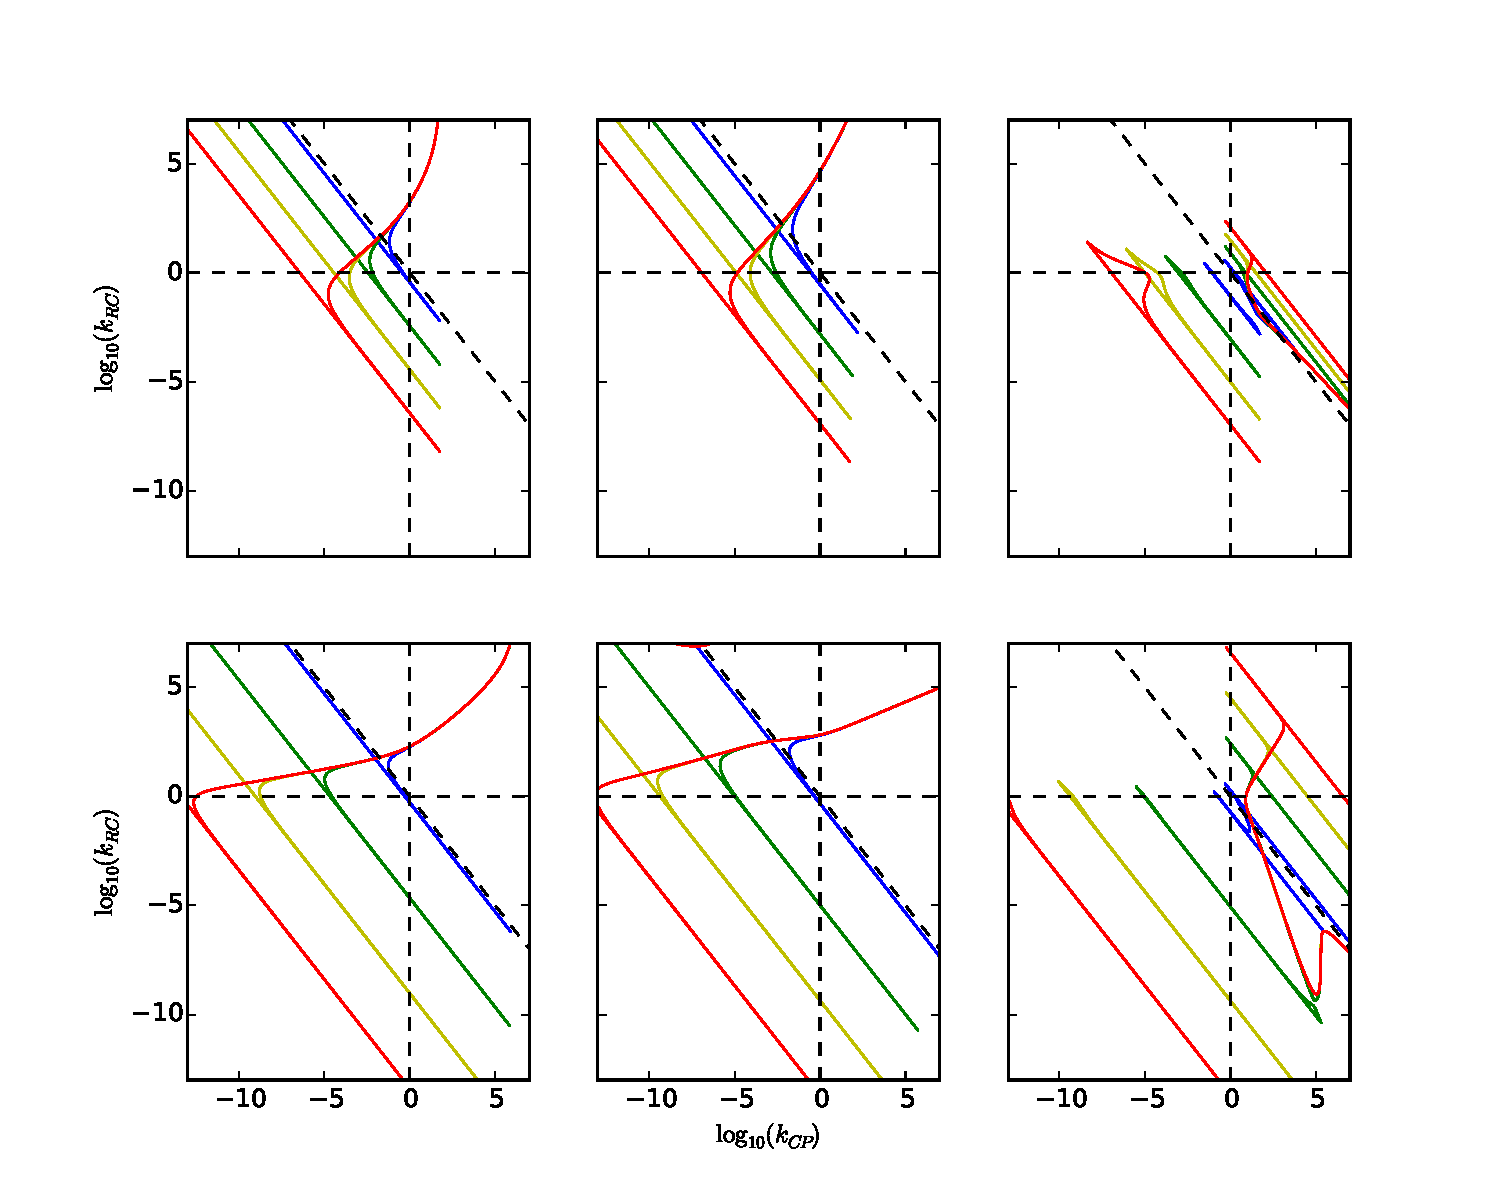
\includegraphics[width = 0.99\textwidth]{./Plots/Z(IC5)AcGrGr.pdf}
  \caption[Env $Z(IC5)$]{\emph{Envolturas de Invasibilidad} para el caso de el depredador intermedio $C$ como invasor frente a una comunidad receptora formada por $R-P$. Las dem\'as especificaciones se comparten con la figura ~\ref{fig:Z(IC2)}.}
  \label{fig:Z(IC5)}
\end{figure}



\subsubsection{\emph{Invasibilidad Mutua}}

La zona de invasi\'on mutua $Z_M$ al ser la interescci\'on de las dos zonas anteriores($Z_{\PP \to \R-\C}$ y $ Z_{\C \to \R-\PP}$, comparte principalmente con $Z(I_{\C \to \PP- \R})$ ,el patr\'on de variaci\'on respecto a cambios en $m_P$, $k_0$ y $\phi$. Adem\'as de ello su forma esta principalmente determinada por $Z(I_{\C \to \PP- \R})$\\
Para $\phi = 2$ y valores elevados de $m_p$ o $k_0$ posee dos componentes conexas, en este caso la diferencia entre $Z_M$ y $Z(I_{\C \to \PP- \R})$ se debe a variaciones en $\vartheta_C^1$ en ambientes de b\'usqueda $2D$ y en $\vartheta_C^2$ en el caso $3D$. Para $\phi = 0.02,0.2$ la diferencia se debe a la presencia de un borde superior el cual reduce la inclusi\'on de comunidades $C_2$ y $C_3$.\\
Adem\'as es notoria la reducci\'on en el \'area total de $Z_M$ con respecto a las anteriores.

\begin{figure}
  \centering
  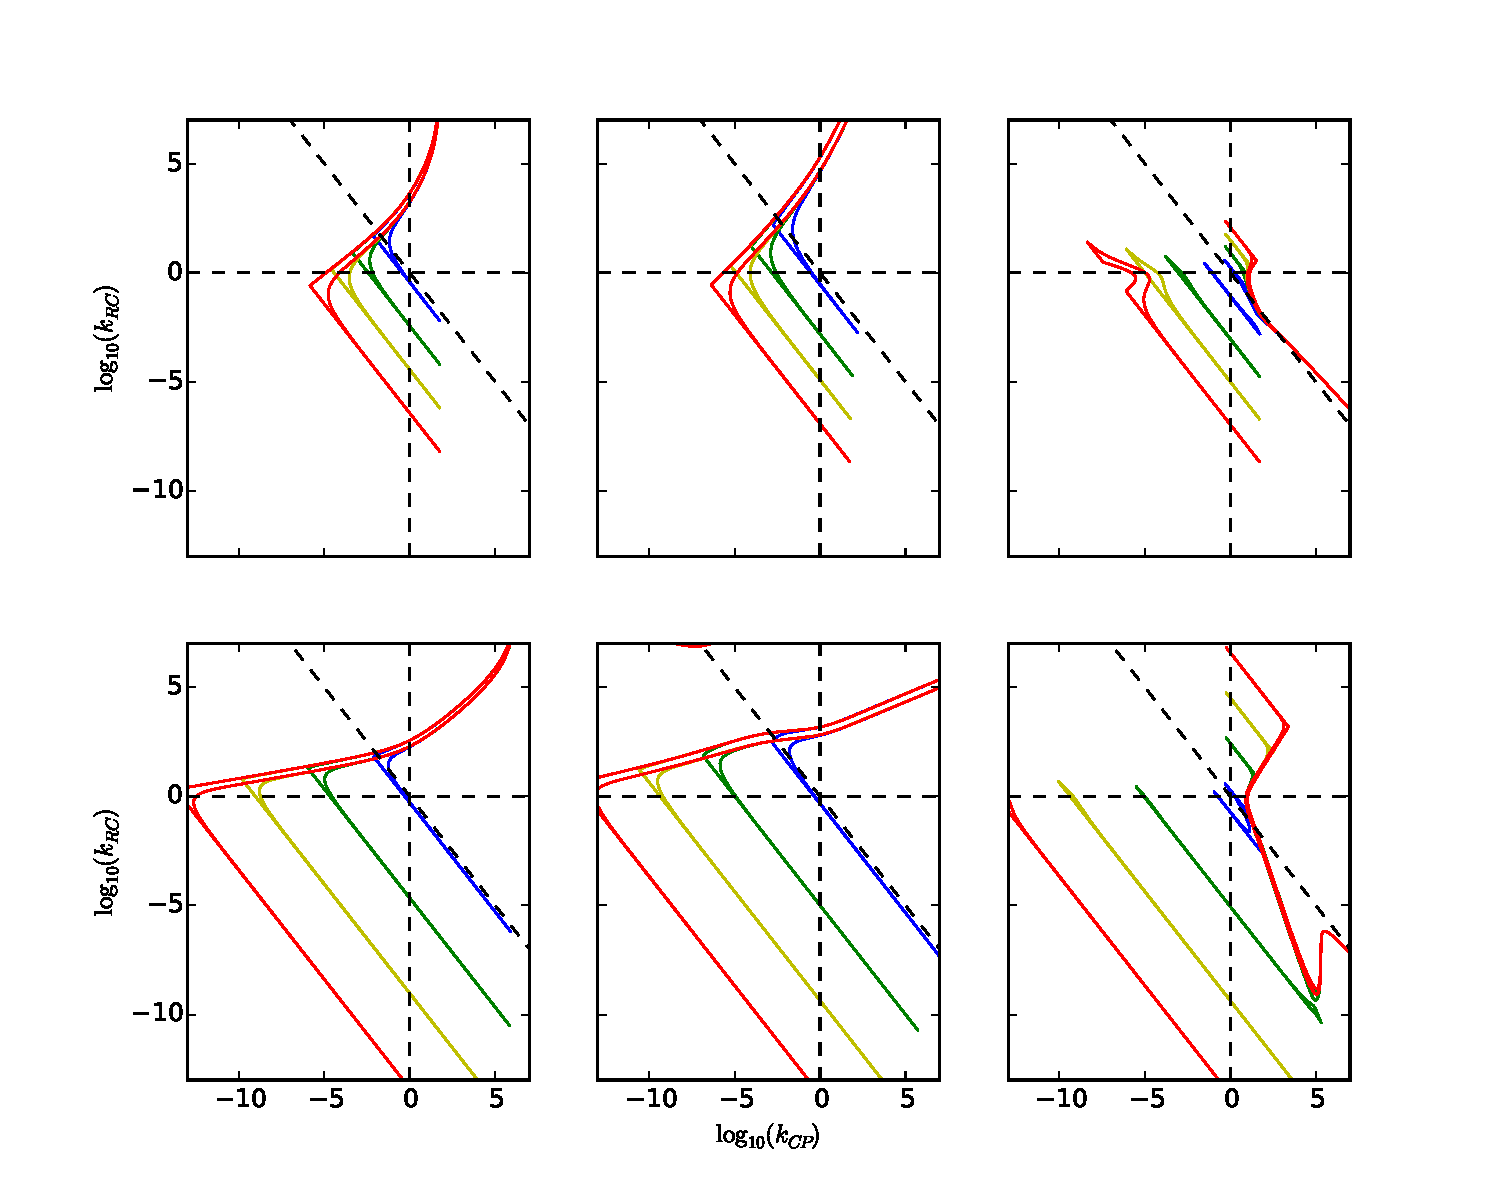
\includegraphics[width = 0.99\textwidth]{./Plots/MutualInvAcGrGr.pdf}
  \caption[Env $I_M$]{\emph{Envolturas de Invasibilidad Mutua} donde ambas sequencias de invasi\'on $S_1$ y $S_2$ dan lugar al m\'odulo completo. Las dem\'as especificaciones se comparten con la figura ~\ref{fig:Z(IC4)}.}
  \label{fig:MutualInv}
\end{figure}

\subsection{Coexistencia}

La regi\'on de coexistencia comparte el comportamiento cualitativo descrito para el caso de la zona de invasibilidad mutua, con su \'area total siendo afectada positivamente por $m_P$ y $k_0$ y $\phi$ afectando principalmente la conectividad de la zona, y generando para $\phi = 2$, dos subzonas diferenciadas principalmente por el valor de $k_{\RP}$ mayor o menor que 1 respectivamente.La distancia entre estas subzonas es afectada posivamente por $m_P$ y $k_0$. \\

A su vez la sub-regi\'on de coexistencia asociada a un equilibrio inestable se ve afectada por $m_P$($k_0$ afecta de manera similar) y $phi$ , donde tenemos que para la zona ``pico'' de inestabilidad(e.g alrededor de $k_0 = 0$ para $m_P = 10^5$ y $\phi = 0.2$) la proporci\'on ocupada respecto a la region total de coexistencia aumenta con respecto a $m_p$ (v\'ease ~\ref{fig:CoexistenceWidth}) ,sin embargo dado que $m_P$ aumenta el \'area total de coexistencia,la proporci\'on inestable en general disminuye con $m_P$($k_0$). Para $\phi = 2$ tenemos que toda el \'area de coexistencia es estable.

\begin{figure}
  \centering
  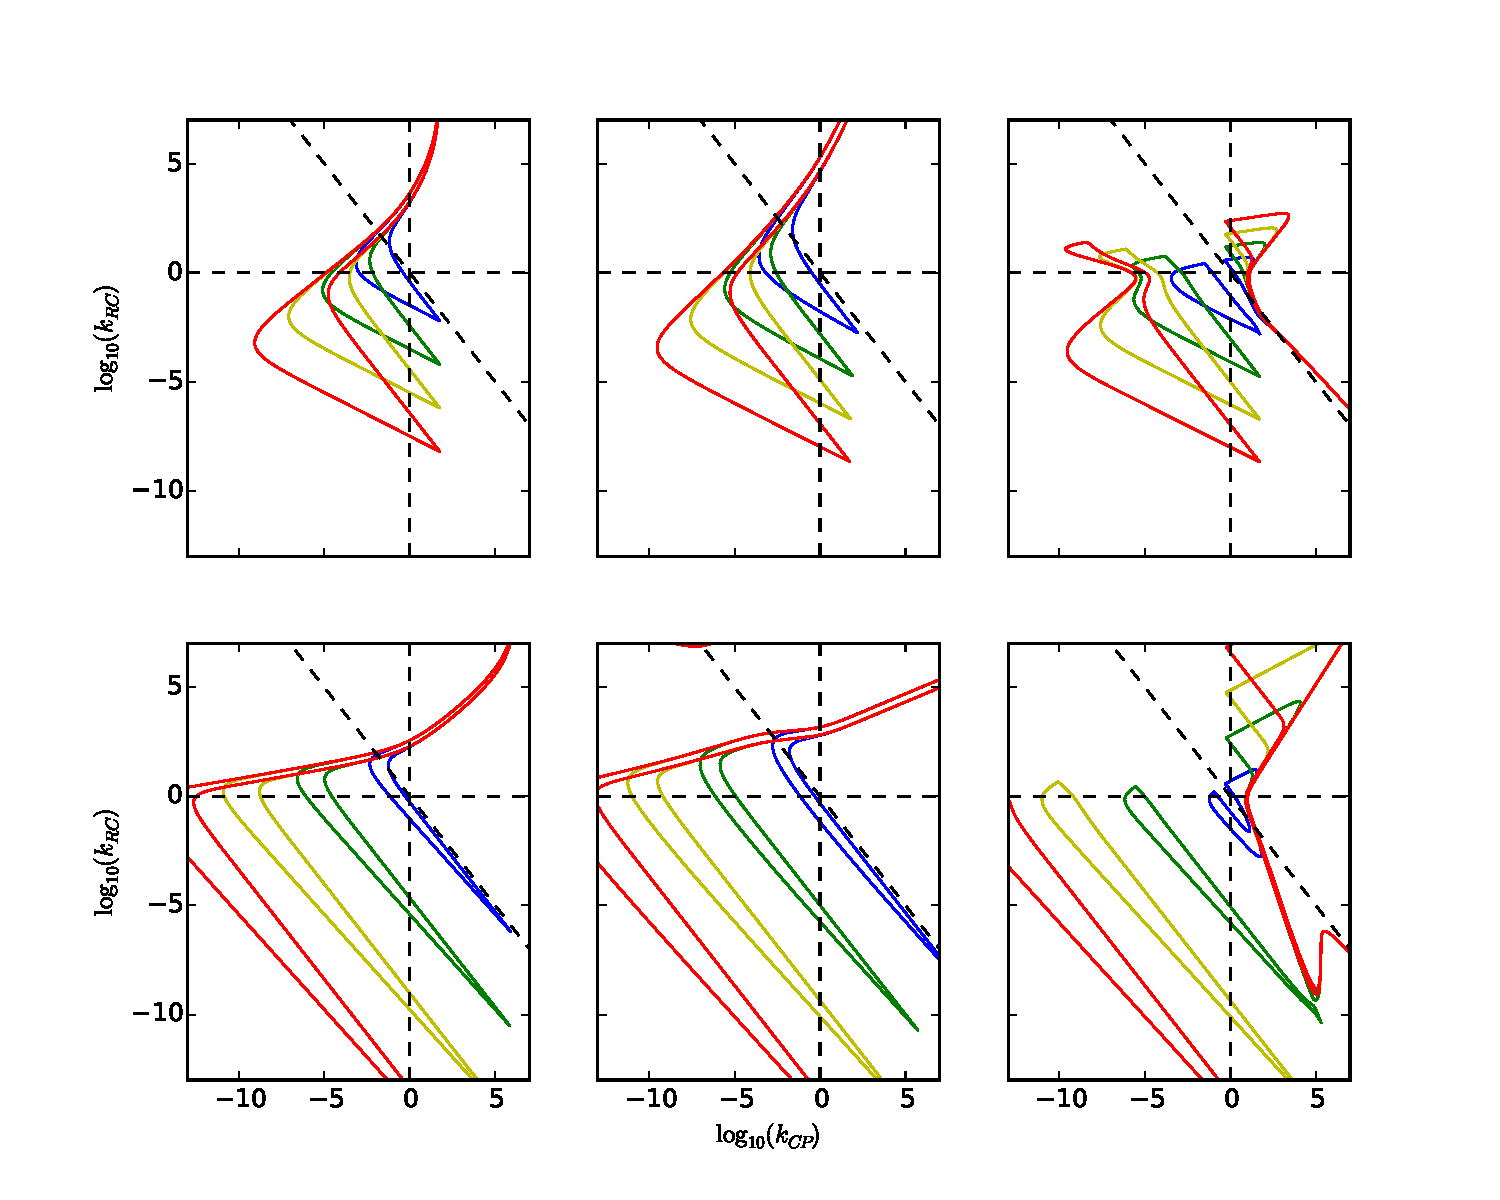
\includegraphics[width = 0.99\textwidth]{./Plots/CoexistenceAcGrGr.pdf}
  \caption[Env $Coexistencia$]{\emph{Coexistencia} donde existe un equilibrio $(R,C,P)$ positivo y este puede ser formado \emph{potencialmente} mediante una secuencia de ensamblaje($S_1$ o $S_2$. Las dem\'as especificaciones se comparten con la figura ~\ref{fig:Z(IC4)}.}
  \label{fig:PSCoexistence}
\end{figure}


\begin{figure}
  \centering
  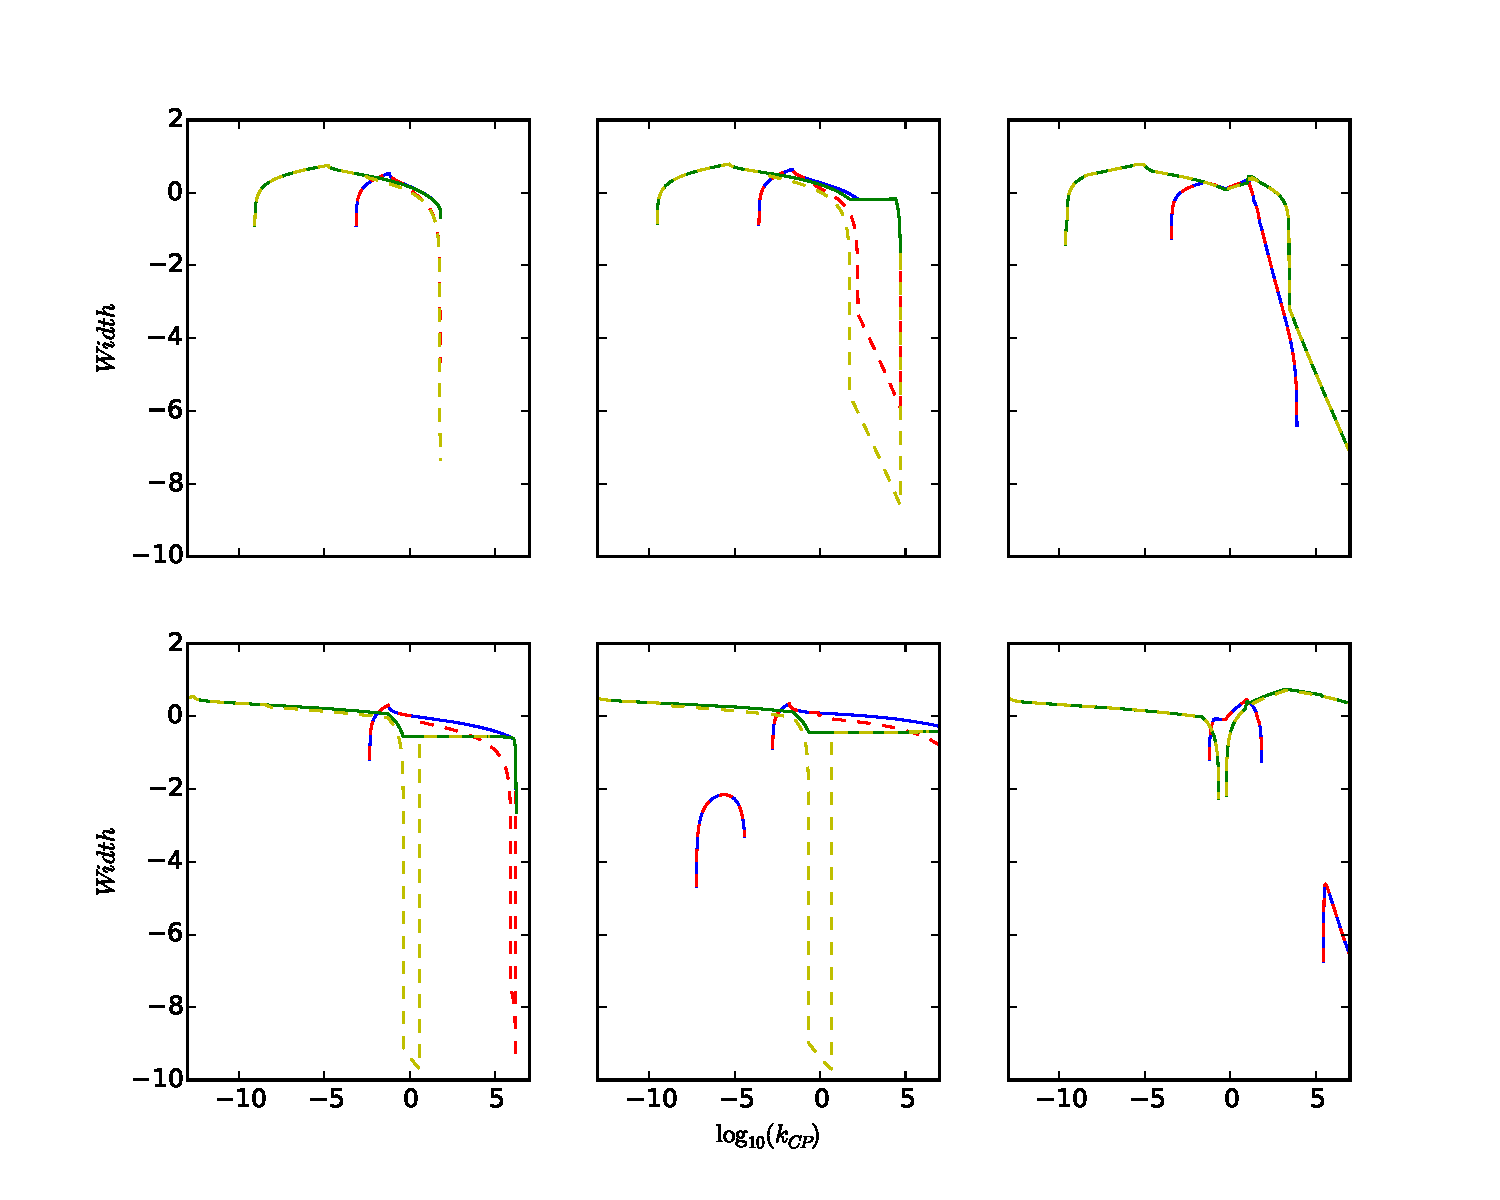
\includegraphics[width = 0.99\textwidth]{./Plots/WidthCoexistenceAcGrGr.pdf}
  \caption[Ancho $Coexistencia$]{Anchos de la zona de \emph{coexistencia} y la zona de \emph{coexistencia estable} respecto a cambios en los valores de $k_{\RC}$.({\hwplotT}) denota \emph{coexistencia} y ({\hwplotK}) \emph{coexistencia estable} . ({\hwplotG}) y  ({\hwplotY}) $10^5 kg$ , ({\hwplotR}) y ({\hwplotB}) para $10^{-10}kg$. Las dem\'as especificaciones se comparten con la figura ~\ref{fig:Z(IC4)}.}
  \label{fig:CoexistenceWidth}
\end{figure}























